% TikZ Asset: FA22GraphTheoryBipartiteMatchingsTikZ-002
%
% Asset ID: FA22GraphTheoryBipartiteMatchingsTikZ-002
% Topic ID: FA22GraphTheoryBipartiteMatchings
% Unit: FA22
% Topic code: FA22-GRAPH
% Related lesson file: FA22_graph_theory_bipartite_matchings_lesson.md
% Related lesson section: Section 9.6 Printable TikZ Hall's Theorem Diagram
%
% Used placeholder:
% [VISUAL PLACEHOLDER: FA22GraphTheoryBipartiteMatchingsTikZ-002 | Source: CCEA FA22-GRAPH-LO004 | Insert from tikz/FA22GraphTheoryBipartiteMatchingsTikZ-002.tex | Purpose: Provide a precise subset-neighbourhood diagram for Hall’s marriage theorem.]
%
% Source:
% CCEA FA22-GRAPH-LO004
%
% Purpose:
% Provide a precise subset-neighbourhood diagram for Hall's marriage theorem.
%
% Creation notes:
% This diagram highlights S = {A, B} on the left and N(S) = {1, 2} on the right.
% It shows the count comparison |S| = 2 and |N(S)| = 2, hence |N(S)| >= |S|.
%
% Off-spec guard:
% This diagram only illustrates Hall's theorem.
% It does not include weighted allocation, cost optimisation or the Hungarian algorithm.

\documentclass[tikz,border=10pt]{standalone}

\usepackage{xcolor}
\usepackage{amsmath}
\usetikzlibrary{positioning,fit,backgrounds}

\definecolor{Canvas}{HTML}{FAF9F6}
\definecolor{Panel}{HTML}{FFFFF0}
\definecolor{Divider}{HTML}{E5E5EA}
\definecolor{AccentGold}{HTML}{D4AF37}
\definecolor{AccentSoftGold}{HTML}{C5A059}
\definecolor{AccentBlush}{HTML}{FBEFEF}
\definecolor{TextColor}{HTML}{2C2C2E}
\definecolor{MutedLine}{HTML}{A9A9B2}

\begin{document}

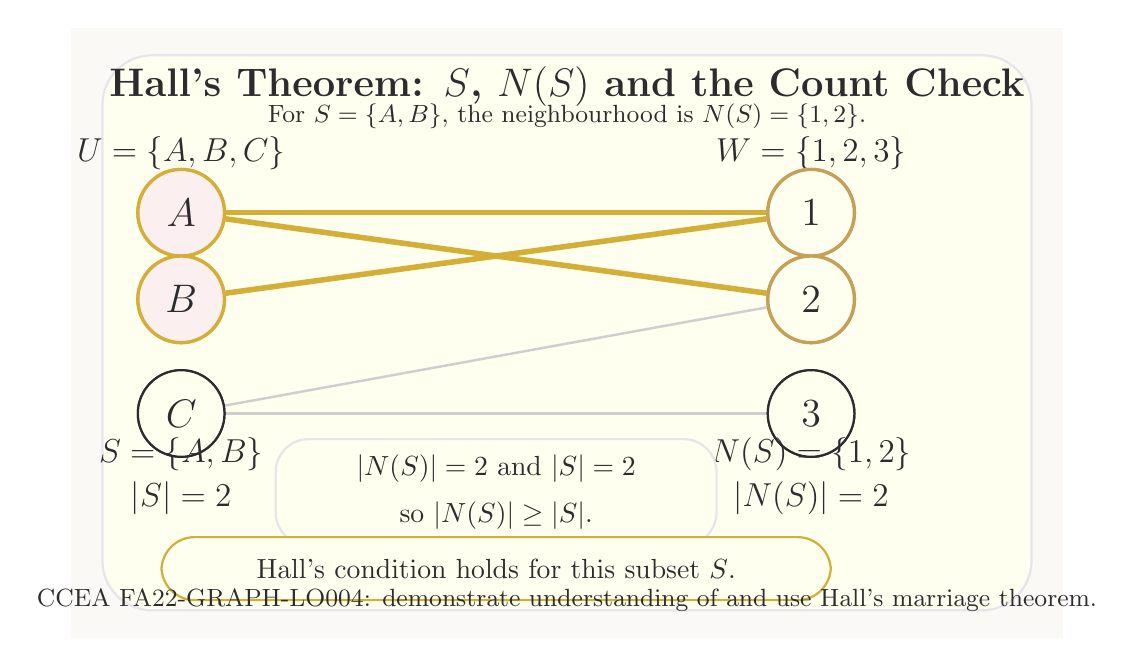
\begin{tikzpicture}[
    vertex/.style={circle, draw=TextColor, fill=Panel, line width=0.8pt, minimum size=11mm, font=\Large\bfseries, text=TextColor},
    selectedvertex/.style={circle, draw=AccentGold, fill=AccentBlush, line width=1.2pt, minimum size=11mm, font=\Large\bfseries, text=TextColor},
    neighbourvertex/.style={circle, draw=AccentSoftGold, fill=Panel, line width=1.2pt, minimum size=11mm, font=\Large\bfseries, text=TextColor},
    setlabel/.style={font=\large\bfseries, text=TextColor},
    smallnote/.style={font=\small, text=TextColor, align=center},
    mathnote/.style={font=\large\bfseries, text=TextColor, align=center},
    inactiveedge/.style={draw=MutedLine, line width=0.9pt, opacity=0.55},
    activeedge/.style={draw=AccentGold, line width=2.0pt},
    subsetbox/.style={draw=AccentGold, fill=AccentBlush, rounded corners=16pt, line width=1.0pt, opacity=0.88},
    neighbourbox/.style={draw=AccentSoftGold, fill=Panel, rounded corners=16pt, line width=1.0pt, opacity=0.9},
    countbox/.style={draw=Divider, fill=Panel, rounded corners=12pt, line width=0.8pt},
    conclusionbox/.style={draw=AccentGold, fill=Panel, rounded corners=12pt, line width=0.8pt}
]

\fill[Canvas] (-1.4,-4.3) rectangle (11.2,3.45);
\draw[draw=Divider, fill=Panel, rounded corners=18pt, line width=0.8pt] (-1.0,-3.95) rectangle (10.8,3.1);

\node[font=\Large\bfseries, text=TextColor] at (4.9,2.7) {Hall's Theorem: \(S\), \(N(S)\) and the Count Check};
\node[smallnote] at (4.9,2.32) {For \(S=\{A,B\}\), the neighbourhood is \(N(S)=\{1,2\}\).};

\node[selectedvertex] (A) at (0,1.1) {$A$};
\node[selectedvertex] (B) at (0,0) {$B$};
\node[vertex] (C) at (0,-1.45) {$C$};

\node[neighbourvertex] (one) at (8,1.1) {$1$};
\node[neighbourvertex] (two) at (8,0) {$2$};
\node[vertex] (three) at (8,-1.45) {$3$};

\node[setlabel] at (0,1.85) {$U=\{A,B,C\}$};
\node[setlabel] at (8,1.85) {$W=\{1,2,3\}$};

\begin{scope}[on background layer]
    \node[subsetbox, fit=(A)(B), inner xsep=12pt, inner ysep=12pt] {};
    \node[neighbourbox, fit=(one)(two), inner xsep=12pt, inner ysep=12pt] {};
\end{scope}

\draw[inactiveedge] (C) -- (two);
\draw[inactiveedge] (C) -- (three);

\draw[activeedge] (A) -- (one);
\draw[activeedge] (A) -- (two);
\draw[activeedge] (B) -- (one);

\node[selectedvertex] at (A) {$A$};
\node[selectedvertex] at (B) {$B$};
\node[vertex] at (C) {$C$};
\node[neighbourvertex] at (one) {$1$};
\node[neighbourvertex] at (two) {$2$};
\node[vertex] at (three) {$3$};

\node[mathnote] at (0,-2.25) {\(S=\{A,B\}\)\\[2pt]\(|S|=2\)};
\node[mathnote] at (8,-2.25) {\(N(S)=\{1,2\}\)\\[2pt]\(|N(S)|=2\)};

\node[countbox, align=center, text=TextColor, minimum width=5.6cm, minimum height=1.35cm] at (4,-2.45)
      {\(\displaystyle |N(S)|=2\) and \(\displaystyle |S|=2\)\\[5pt]
       so \(\displaystyle |N(S)|\ge |S|\).};

\node[conclusionbox, align=center, text=TextColor, minimum width=8.5cm, minimum height=0.8cm] at (4,-3.42)
      {Hall's condition holds for this subset \(S\).};

\node[smallnote] at (4.9,-3.82) {CCEA FA22-GRAPH-LO004: demonstrate understanding of and use Hall's marriage theorem.};

\end{tikzpicture}

\end{document}
